\documentclass{chi-ext}
% Please be sure that you have the dependencies (i.e., additional LaTeX packages) to compile this example.
% See http://personales.upv.es/luileito/chiext/

%% EXAMPLE BEGIN -- HOW TO OVERRIDE THE DEFAULT COPYRIGHT STRIP -- (July 22, 2013 - Paul Baumann)
% \copyrightinfo{Permission to make digital or hard copies of all or part of this work for personal or classroom use is granted without fee provided that copies are not made or distributed for profit or commercial advantage and that copies bear this notice and the full citation on the first page. Copyrights for components of this work owned by others than ACM must be honored. Abstracting with credit is permitted. To copy otherwise, or republish, to post on servers or to redistribute to lists, requires prior specific permission and/or a fee. Request permissions from permissions@acm.org. \\
% {\emph{CHI'14}}, April 26--May 1, 2014, Toronto, Canada. \\
% Copyright \copyright~2014 ACM ISBN/14/04...\$15.00. \\
% DOI string from ACM form confirmation}
%% EXAMPLE END -- HOW TO OVERRIDE THE DEFAULT COPYRIGHT STRIP -- (July 22, 2013 - Paul Baumann)

\title{Exploiting Publication Contents and Collaboration Networks for Collaborator Recommendation}
\numberofauthors{6}
% Notice how author names are alternately typesetted to appear ordered in 2-column format;
% i.e., the first 4 autors on the first column and the other 4 auhors on the second column.
% Actually, it's up to you to strictly adhere to this author notation.
\author{
  \alignauthor{
  	\textbf{Zhen Chen}\\
  	\affaddr{School of Software}\\
  	\affaddr{Dalian University of Technology, China}\\
  	\email{zhenchentl@outlook.com}
  }\alignauthor{
  	\textbf{Feng Xia}\\
  	\affaddr{School of Software}\\
  	\affaddr{Dalian University of Technology, China}\\
  	\email{f.xia@acm.org}
  }
  \vfil
  \alignauthor{
  	\textbf{Huizhen Jiang}\\
  	\affaddr{School of Software}\\
  	\affaddr{Dalian University of Technology, China}\\
  	\email{huizhen.jiang@gmail.com}
  }\alignauthor{
  	\textbf{Tie Qiu}\\
  	\affaddr{School of Software}\\
  	\affaddr{Dalian University of Technology, China}\\
  	\email{qiutie@dlut.edu.cn}
  }
  \vfil
  \alignauthor{
  	\textbf{Haifeng Liu}\\
  	\affaddr{School of Software}\\
  	\affaddr{Dalian University of Technology, China}\\
  	\email{haif.liu@hotmail.com}
  }
%\alignauthor{
%  	\textbf{Nana Yaw Asabere}\\
%  	\affaddr{School of Software}\\
%  	\affaddr{Dalian University of Technology, China}\\
%  	\email{yawasabere2005@yahoo.com}
%  }
}

% Paper metadata (use plain text, for PDF inclusion and later re-using, if desired)
\def\plaintitle{CHI LaTeX Extended Abstracts Template}
\def\plainauthor{Luis A. Leiva}
\def\plainkeywords{Collaboration recommendation, publication contents, collaboration networks, topic clustering, random walk.}
\def\plaingeneralterms{Documentation, Standardization}

\hypersetup{
  % Your metadata go here
  pdftitle={\plaintitle},
  pdfauthor={\plainauthor},
  pdfkeywords={\plainkeywords},
  pdfsubject={\plaingeneralterms},
  % Quick access to color overriding:
  %citecolor=black,
  %linkcolor=black,
  %menucolor=black,
  %urlcolor=black,
}

\usepackage{graphicx}   % for EPS use the graphics package instead
\usepackage{balance}    % useful for balancing the last columns
\usepackage{bibspacing} % save vertical space in references
\usepackage{subfigure}
\usepackage{epstopdf}


\begin{document}

\maketitle

\begin{abstract}
Due to the expansion of academic research in diverse fields, the problem of finding relevant and potential collaborators has become cumbersome. In this work, we propose an academic collaboration recommendation model called CCRec. CCRec combines publication contents with collaboration networks to effectively generate academic collaboration recommendation for researchers. Using the DBLP data sets, we conduct benchmarking experiments to examine the performance of CCRec. Our preliminary experimental results show that CCRec outperforms other state-of-the-art methods especially in addressing the topic drift problems.

\end{abstract}

\keywords{\plainkeywords}
%\textcolor{red}{Mandatory section to be included in your final version.}

\category{H.5.m}{Information interfaces and presentation (e.g., HCI)}{Miscellaneous}.
%See \cite{ACMCCS}
%See: \url{http://www.acm.org/about/class/1998/}
%for help using the ACM Classification system.
%\textcolor{red}{Mandatory section to be included in your final version.}

%\terms{\plaingeneralterms}
%\textcolor{red}{Optional section to be included in your final version.}


% =============================================================================
\section{Introduction}
% =============================================================================
A collaboration network is a type of academic social networks formed by researchers and their collaborations. In academia, recommending collaborators to different researchers (groups) may help researchers build more collaborations and become more prolific.

Some existing research studies \cite{benchettara2010supervised} \cite{brandao2012affiliation} \cite{brandao2013using} have proposed the utilization of affiliations to exploit collaboration networks and profiles of researchers for academic collaboration recommendation. However, one important factor that has been consistently ignored by researchers is that collaborations among researchers largely depend on the research field reflected from their publications. Consequently, improved academic collaboration recommendation can be achieved through the combination of publication contents and collaboration networks.

In this work we propose an academic collaboration recommendation model called CCRec. CCRec combines publication contents with collaboration networks to effectively generate academic collaboration recommendation for researchers. CCRec first uses topic clustering to partition the words from all the publications' titles into multiple domains. Then, CCRec computes the degree of interest (DoI) and the strength of influence (SoI) pertaining to each domain for each researcher. Finally, DoI and SoI are combined to form the feature vector for each researcher. By comparing the similarity of feature vector, CCRec provides a TopN collaboration recommendation list.


% =============================================================================
\section{PROPOSED SCHEME}
% =============================================================================
Our proposed design scheme for CCRec is inspired by the reality and truth that a researcher usually desires to know other researchers who have similar research interests. As mentioned above, researchers often behave differently across multiple domains of interests. Such behaviors usually reveal academic features of different researchers in the network. In this work, we define the DoI and SoI for researchers in different domains. Furthermore, we use the feature vector combined by DoI and SoI to evaluate the similarity of researchers and then obtain the recommendation list.

%proposed a content based method to measure the "attention-degree" of researchers on different domains by parsing papers' title, and a graph based method to measure the %"influence-strength" by analysis the coauthor networks. Additionally, we merge the two metrics into "membership-degree" to measure the researchers academic interest feature. Finally, %we make a TopN recommendation based on the similarity of researchers' membership-degree vectors.

\begin{figure}
\centering
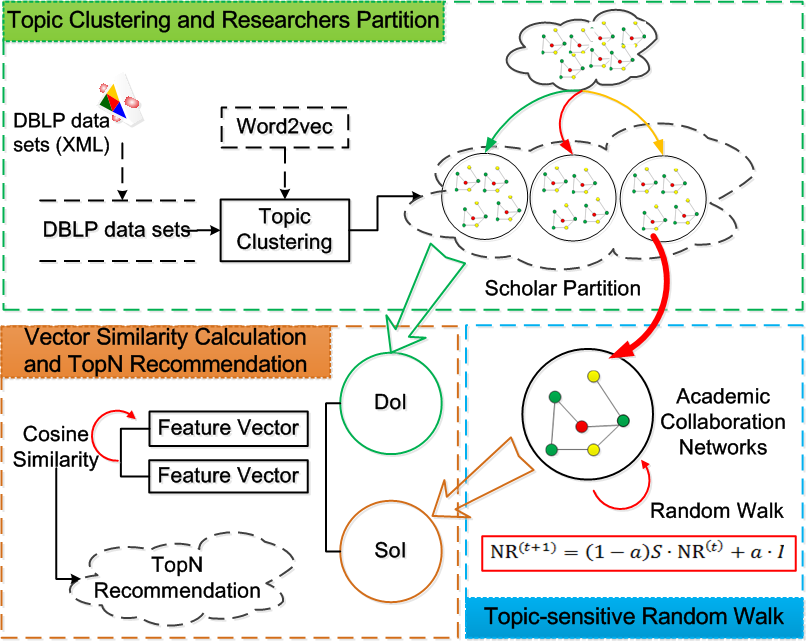
\includegraphics [width=3.4in]{Fig1.png}
\caption{The architecture diagram of CCRec model}
\end{figure}

Figure 1 depicts the three components of CCRec. Topic clustering and researcher partition distribute researchers according to multiple domains and acquire a DoI for each researcher. Topic-sensitive random walk calculates the SoI in each domain, and the TopN recommendation provides the recommendation list.

\subsection{Topic Clustering and Researcher Partition}
% -----------------------------------------------------------------------------
In CCRec, topic clustering and researcher partition generate various domains and map all researchers into these domains. Initially, CCRec extracts keywords from titles of all the papers for each researcher, and filters out some irrelevant words, e.g. "of","the", "and", etc. As core contents in a paper, preprocessed keywords in CCRec are signified as valuable and reliable data in a variety of academic topics. We use word2vec, a famous tool of NLP (Natural Language Processing) to cluster the keywords into various domains. Then, if some keywords of a researcher belong to a domain, we will partition the researcher to that particular domain. We emphasize that one researcher always belongs to several domains and there are also many researchers in one domain.

\subsection{Feature Vector Calculation}
% -----------------------------------------------------------------------------
To measure the distribution of researchers' interests, we define DoI as researcher's proportion of interest in one domain:
\begin{equation}
DoI_{s,d}=\frac{N_{d}}{\sum_{k=1}^{n} N_{k}}
\end{equation}
where $N_{d}$ is the number of keywords of researcher $s$ in domain $d$. It is a content-based method that utilizes the information on the titles of researchers' publications.

We define SoI as researcher's strength of influence in one domain, which is measured by a topic-sensitive random walk method based on collaboration networks. The core equation of the random walk method is shown below:
\begin{equation}
R_{d}^{(t+1)}=\alpha \mathbf{S}R_{d}^{(t)}+(1-\alpha)q
\end{equation}
where $R_{d}$ represents the rank score vector of all researchers in domain $d$, $q$ is the initial vector $R^0$, and $\alpha$ denotes the damping coefficient. Random walk is an iterative process. After limited iterations, the vector $R$ will be convergent. The vector item in this scenario is defined as SoI. We therefore obtain SoI through $SoI_{s}=R_{d,s}$.

To be more specific, we define feature vector $F$ by combining $DoI$ and $SoI$, which measures the academic feature of researchers in various domains.

\begin{equation}
F_{s,d}=DoI_{s}*SoI_{s}
\end{equation}

\subsection{Collaboration Recommendation by Feature Vector Similarity}
% -----------------------------------------------------------------------------
In CCRec, the academic features of researchers are measured by the feature vector $F$. We use a \emph{cosine similarity} method to compute the similarity of these feature vectors, and further compute the similarity between researchers.
\begin{equation}
Sim(s_{1},s_{2})=\frac{\sum_{i=1}^{n}(F_{s_{1},i}*F_{s_{2},i})}{\sqrt{\sum_{i=1}^{n}F_{s_{1},i}^2}*\sqrt{\sum_{i=1}^{n}F_{s_{2},i}^2}}
\end{equation}

Finally, CCRec recommends potential academic collaborators to researchers who have common interests and high similarities, by providing a TopN recommendation list for each researcher in the network.
% =============================================================================
\section{Evaluation and Analysis}
% =============================================================================
\begin{figure*}
\centering
\subfigure[Precision]{
\label{fig:2-a}
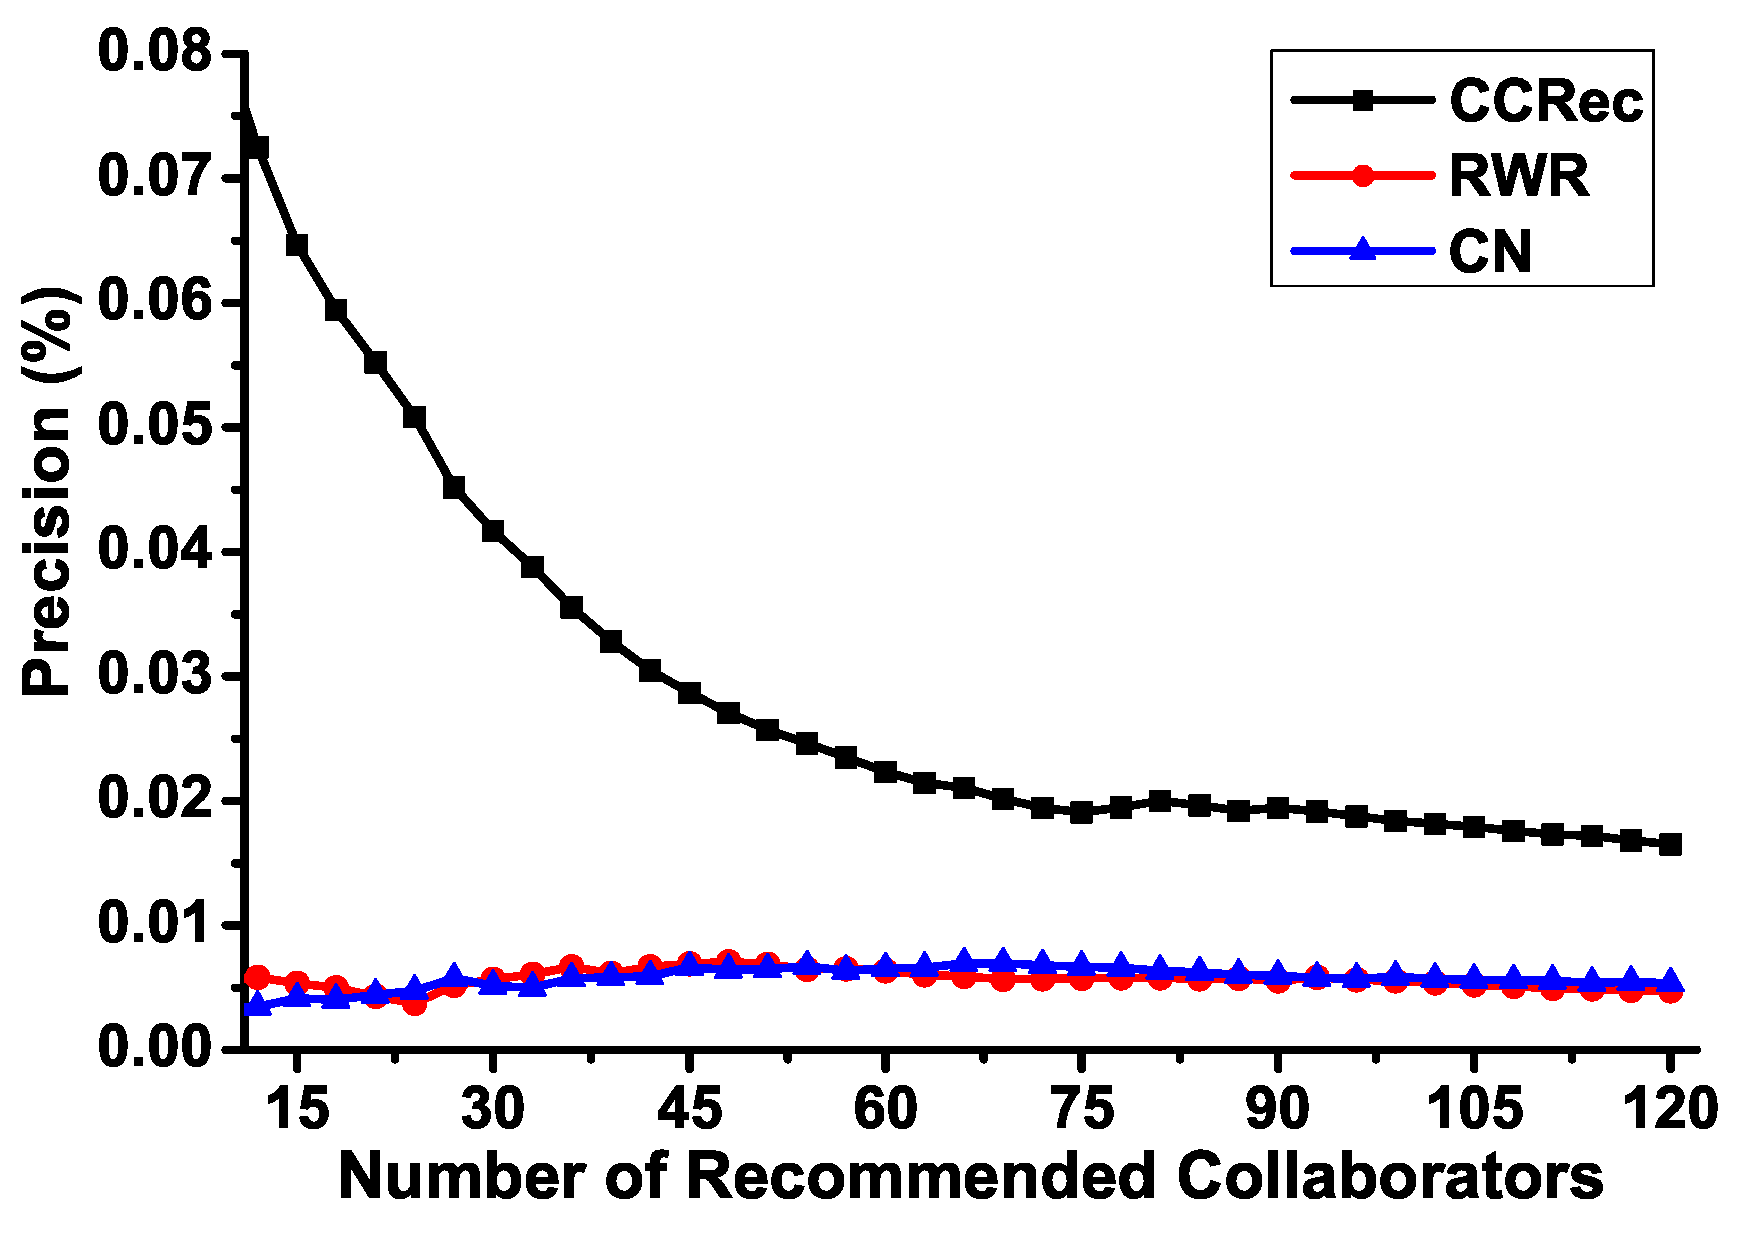
\includegraphics[width=0.32\textwidth]{Fig2-a.eps}}
\subfigure[Recall Rate]{
\label{fig:2-b}
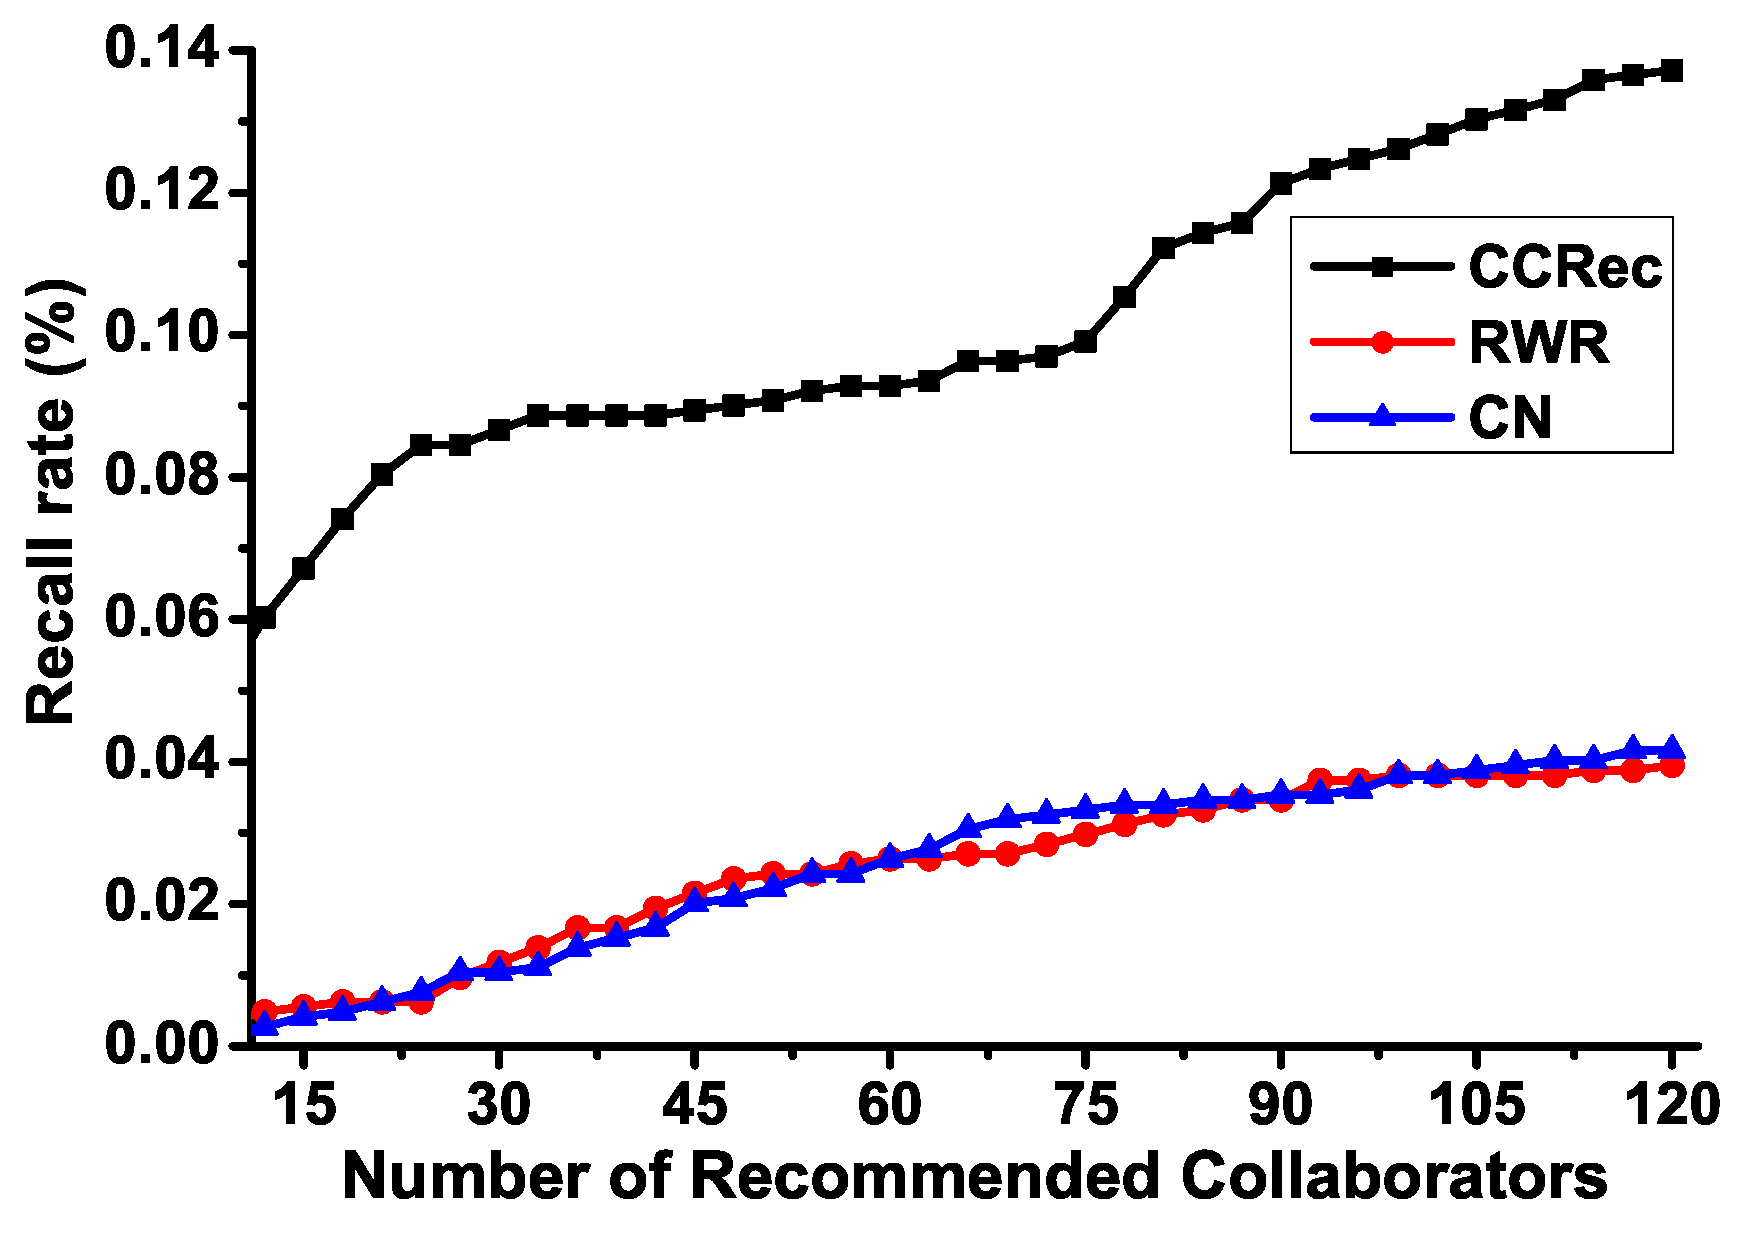
\includegraphics[width=0.32\textwidth]{Fig2-b.eps}}
\subfigure[F1]{
\label{fig:2-c}
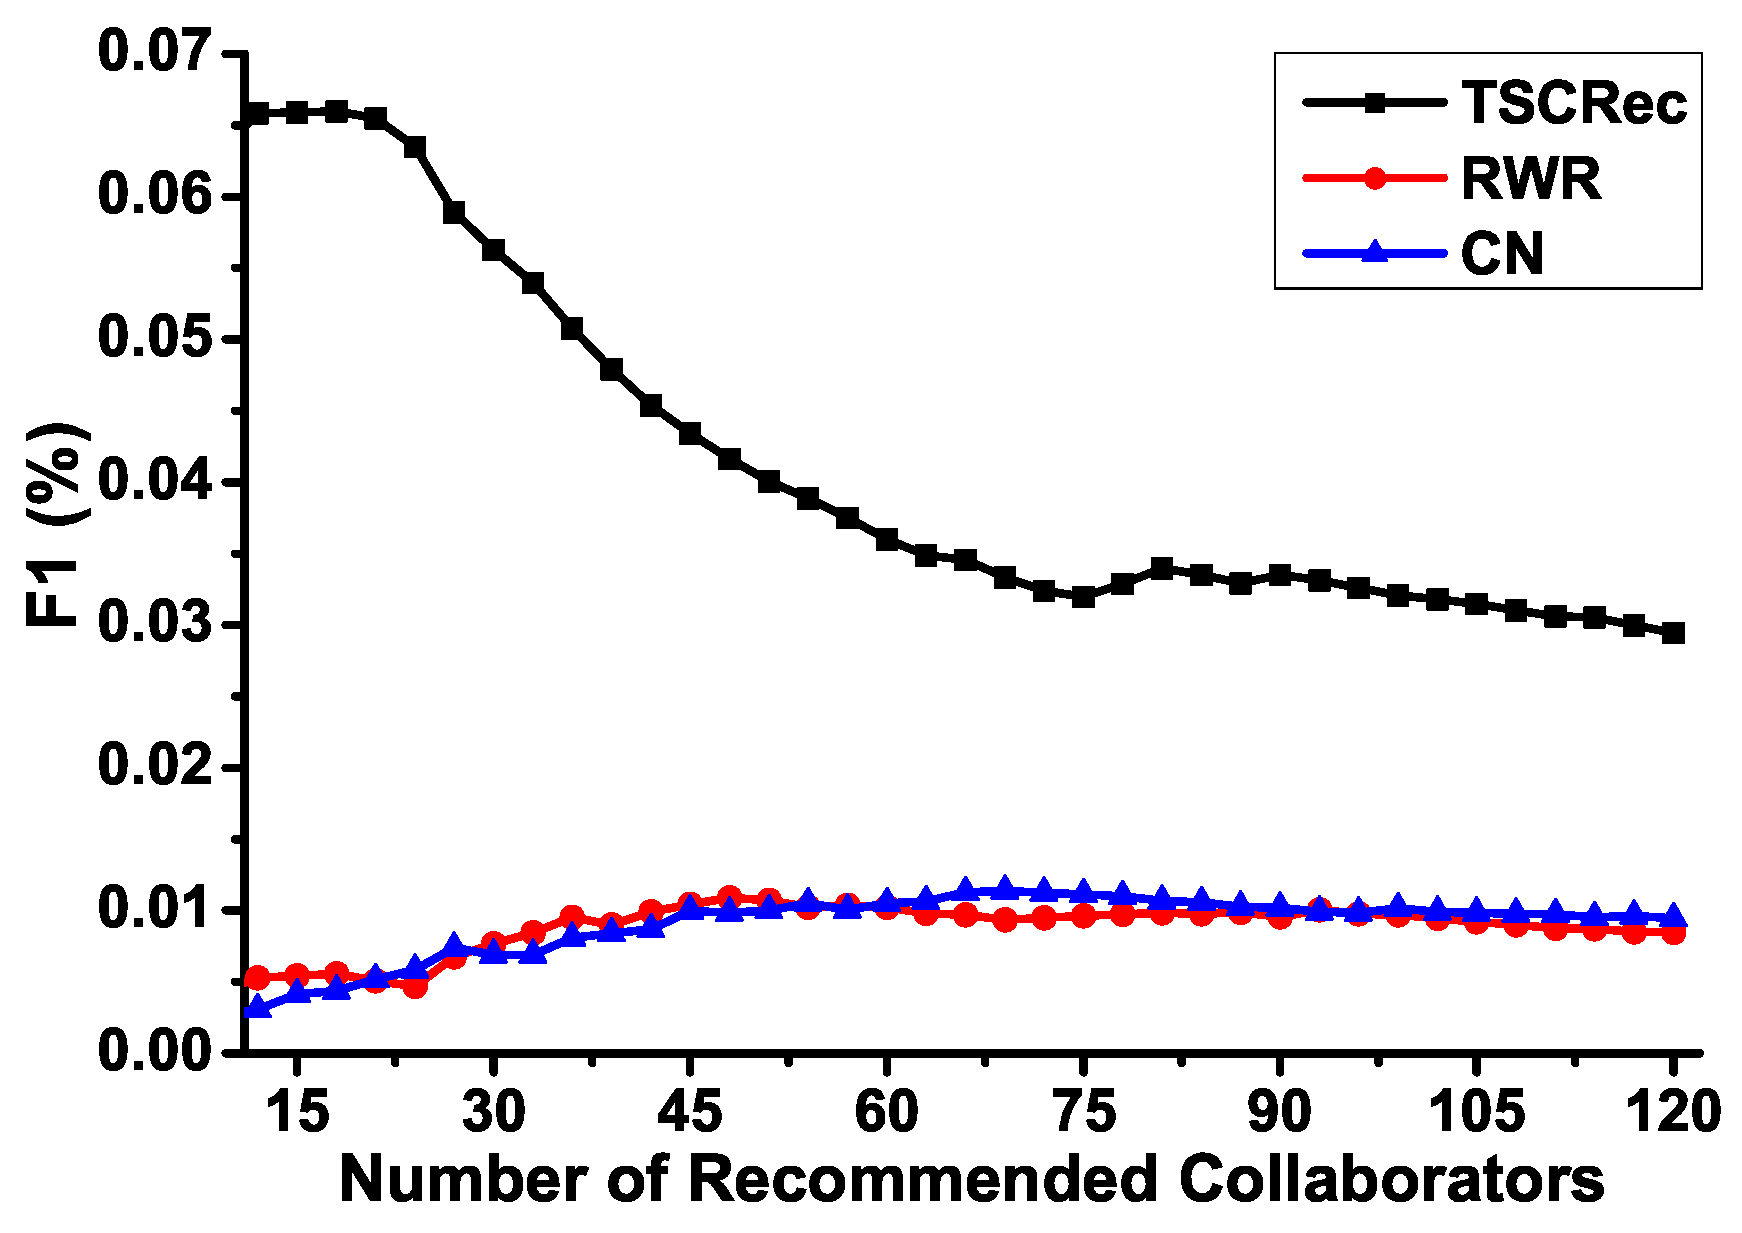
\includegraphics[width=0.32\textwidth]{Fig2-c.eps}}
\caption{Performance of CCRec, RWRec and CNRec}
\label{fig:5}       % Give a unique label
\end{figure*}
Using a subset of DBLP dataset relevant to data mining, we embarked on benchmarking experiments to evaluate the performance of CCRec. We took the year 2011 as the partition time of training and testing sets. To evaluate our model in a better way, we compared CCRec with the two following approaches. RWRec: a random walk recommendation model based on collaboration networks. CNRec: a common neighbors based recommendation model \cite{lopes2010collaboration}. We adopted three metrics to evaluate the performance of CCRec: precision, recall rate and F1. We recommend the new collaborators who never cooperated with the target researcher, because the new collaborators are more meaningful and practical in academia.

Figure 2 shows the performance of CCRec, RWRec and CNRec in terms of precision, recall rate and F1 with the number of recommended collaborators increasing. It can be observed that CCRec significantly outperforms RWRec and CNRec all the time in these three metrics. CCRec shows a downtrend for precision and an uptrend for recall rate. In the case of F1, it reaches the peak 6.598\% when recommending 18 researchers.

In a nutshell, CCRec outperforms RWRec and CNRec with higher precision, recall rate and F1. This is because CCRec combines publication contents and collaboration networks which has a distinct advantage in recommending new collaborators.

% =============================================================================
\section{Conclusion}
% =============================================================================
The conclusions we reach are: 1) CCRec outperforms RWRec and CNRec in precision, recall rate and F1 integrating publication contents with academic collaboration networks. 2) With topic clustering, the problem of topic drift has been well solved.

Our research on CCRec reveals that the combination of information regarding publication contents and collaboration networks of researchers can improve the generation of effective academic collaborations.

\balance
\bibliographystyle{acm-sigchi}
\bibliography{CCRec}

\end{document}
